% 
% Procedure
% @author Pieter Maene <pieter.maene@student.kuleuven.be>
%

\chapter{Procedure}
\label{chap:procedure}

Dit hoofdstuk geeft de procedure die in Helios gevolgd moet worden om een verkiezing met threshold encryptie op te zetten. In \ref{sec:proc:voorbereiding} wordt bekeken welke informatie gekend moet zijn voordat met het aanmaken van de verkiezing aangevat wordt. De procedure van Helios wordt in \ref{sec:proc:helios} beschreven.

\section{Voorbereiding}
\label{sec:proc:voorbereiding}

\subsection{Trustees}

%TODO Referentie naar Threshold in Helios

De trustees zijn de personen die verantwoordelijk zullen zijn voor het decrypteren van het resultaat. Aangezien zijn een belangrijke rol spelen in het verkiezingsproces, is het belangrijk vooraf vast te leggen wie dit zal doen. Helios heeft ondersteuning voor threshold encryptie. Er moet dus ook nagedacht worden over het threshold schema: hoeveel trustees nodig zullen zijn om het resultaat van de verkiezing te decrypteren. Om een trustee aan te maken, moeten zijn naam en een geldig e-mailadres opgegeven worden.

\subsection{Vragen}
\label{sec:proc:voorbereiding:vragen}

Het belangrijkste van de verkiezing zijn uiteraard de vragen die de kiezers zullen moeten beantwoorden. Bij elke vraag kan in Helios aangegeven worden hoeveel antwoorden elke kiezer kan aanduiden, dus ook dit moet op voorhand bepaald worden. Het resultaat kan ofwel absoluut ofwel relatief weergegeven worden. In het eerste geval zal bij elke optie het aantal stemmen voor deze optie getoond worden, in het tweede alleen de relatieve plaatsen van de opties onderling.

\subsection{Kiezers}
\label{sec:proc:voorbereiding:kiezers}

Een verkiezing in Helios kan opengesteld worden voor iedereen of voor specifieke kiezers. Bij een gesloten verkiezing moet op voorhand een lijst van geldige kiezers opgesteld worden.

\npar Deze kiezers kunnen in Helios ge\"importeerd worden door een CSV-bestand aan te maken. Helios heeft van elke kiezer de volledige naam en een uniek ID nodig. Het e-mailadres van de kiezer kan opgegeven worden, maar dit is niet vereist. Er kan ook aangegeven worden welk authenticatiesysteem (bv. Google of Shibboleth) gebruikt wordt door de kiezer. Wanneer dit laatste veld leeg is, zal een gegenereerd wachtwoord naar hem opgestuurd worden.

\section{Helios}
\label{sec:proc:helios}

\subsection{Aanmaken van de verkiezing}

De eerste stap is het aanmaken van de verkiezing. Hier moet eerst de basisinformatie van de verkiezing opgegeven worden zoals de naam en het type verkiezing. Ofwel kan er een verkiezing aangemaakt worden, ofwel een referendum. Voor beide types is de procedure echter identiek.

\begin{figure}
  \center{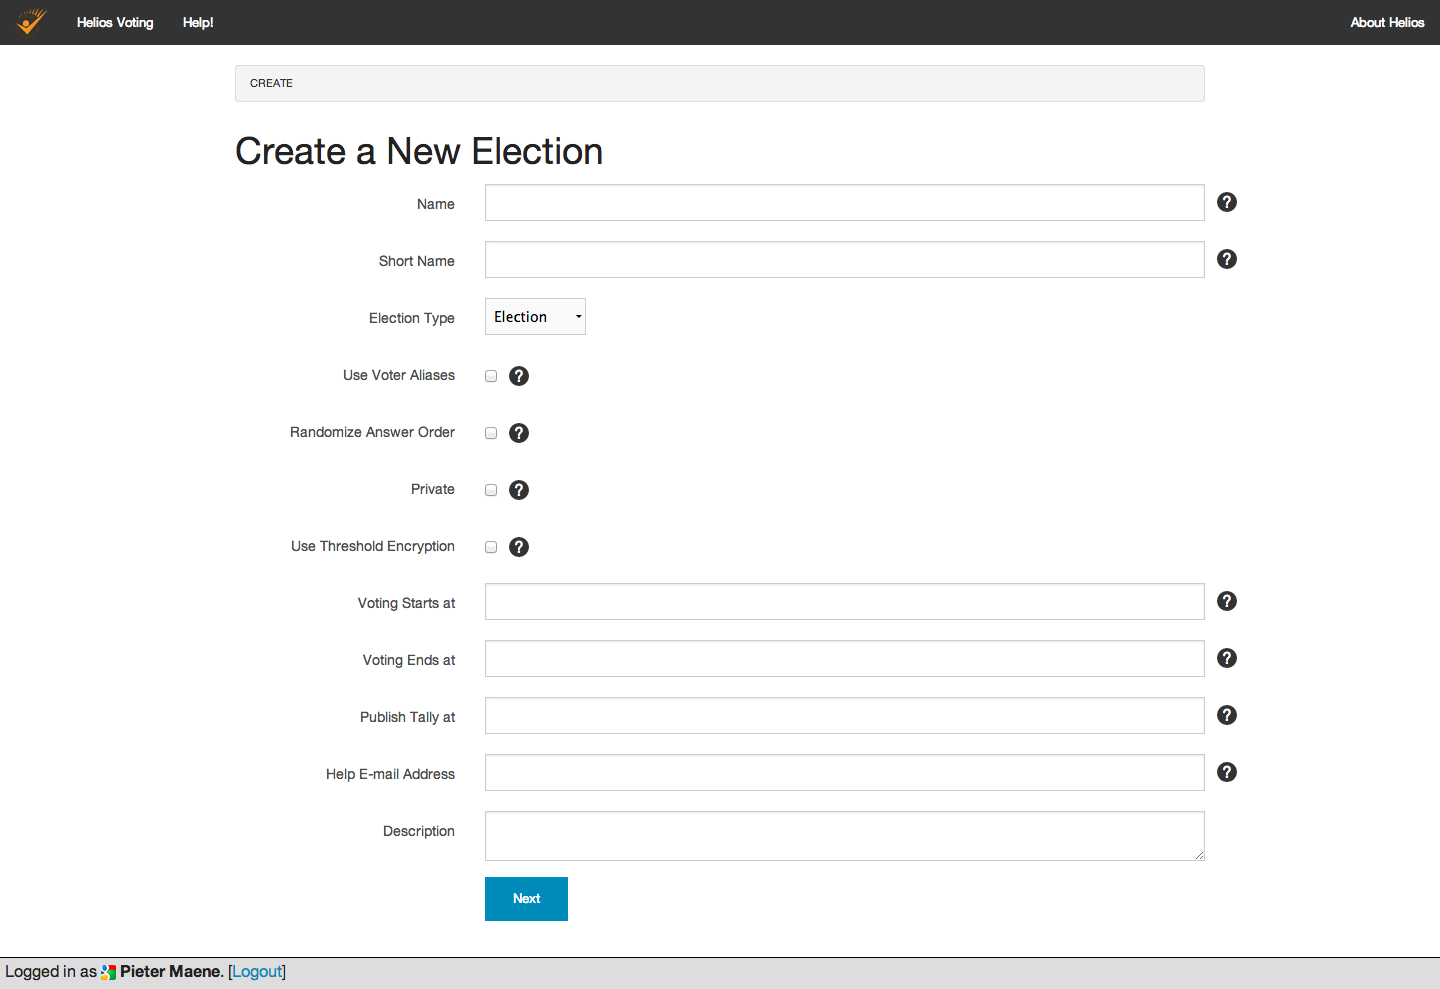
\includegraphics[width=0.9\linewidth]{proc/elections_new.png}}
  \caption{Create a new Election}
  \label{fig:proc:elections_new}
\end{figure}

%TODO Referentie naar BTC in Helios

\npar Vervolgens kunnen een aantal belangrijke functies aan- of uitgezet worden. Wanneer aliassen gebruikt worden, dan worden de namen van de kiezers verborgen in het publieke ballot tracking center. Het is ook mogelijk om de antwoorden in een random volgorde op het biljet te laten zetten. Bij een geheime verkiezing kan alleen bekeken worden door de geregistreerde kiezers. Hier moet ook aangegeven worden of threshold encryptie gebruikt zal worden.

\npar Tot slot is het mogelijk om aan te geven wanneer de verkiezing moet starten en sluiten. Wanneer het resultaat niet onmiddellijk na het aflopen van de verkiezing gepubliceerd mag worden, kan een alternatief tijdstip hiervoor opgegeven worden.

\subsection{Trustees}

%TODO Referentie naar Dashboard in Interface

Eens de nieuwe verkiezing aangemaakt is, moeten de trustees toegevoegd worden. Deze stap is eerst gezet in de procedure omdat hij veruit de meeste tijd in beslag neemt. De beheerder van de verkiezing moet eerst alle trustees aanmaken. De trustee krijgt dan ook meteen een link toegestuurd via e-mail naar zijn trustee dashboard waar hij al zijn acties zal moeten uitvoeren.

\begin{figure}
  \center{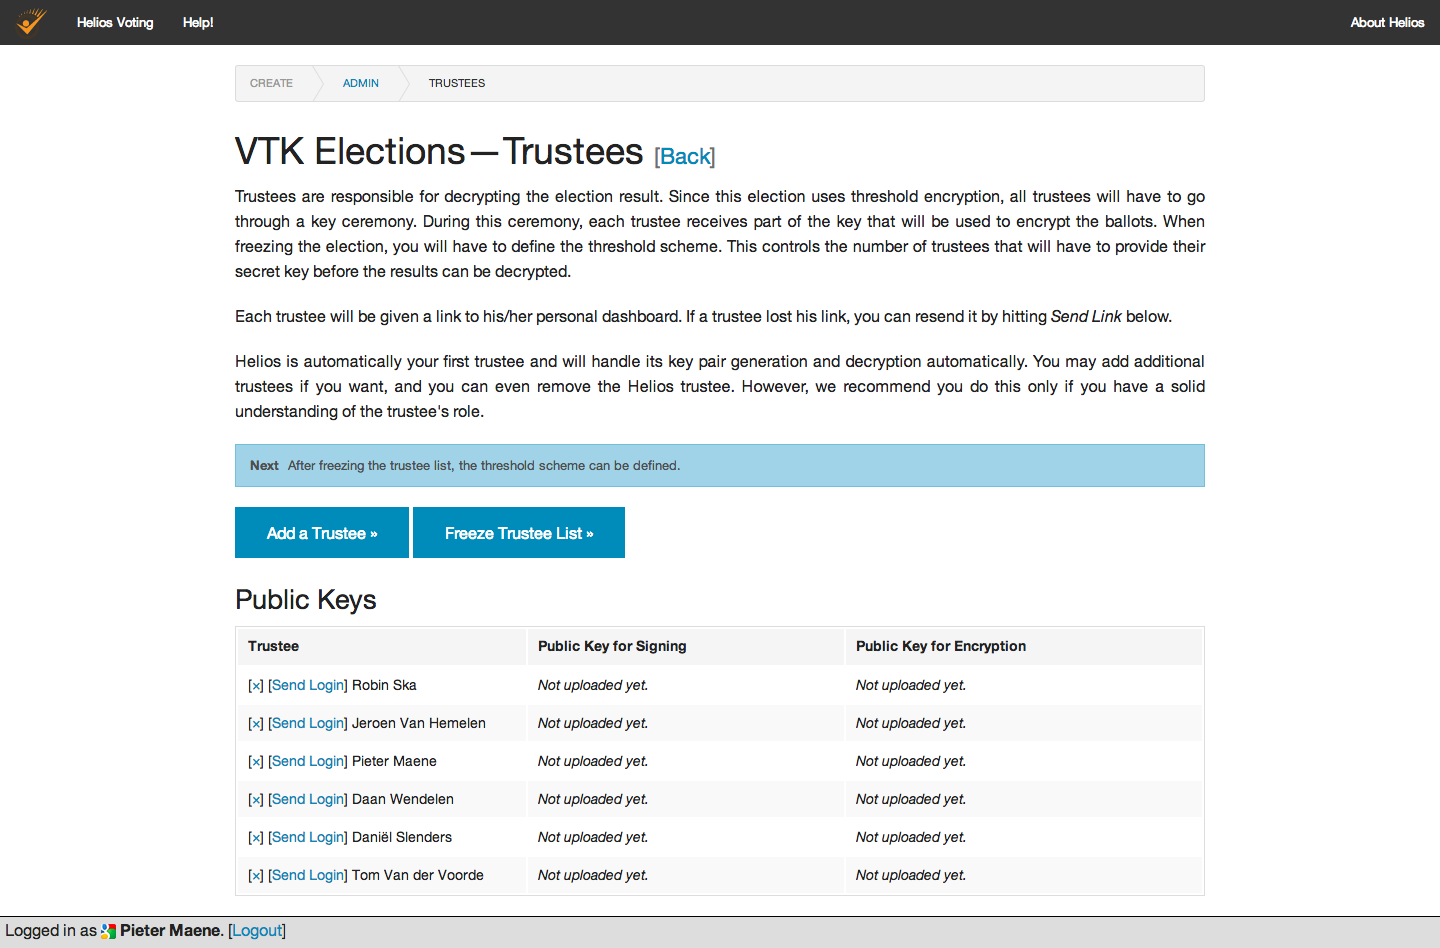
\includegraphics[width=0.9\linewidth]{proc/trustees_view.png}}
  \caption{Trustees}
  \label{fig:proc:trustees_view}
\end{figure}

\subsubsection{Verkiezing zonder threshold encryptie}

%TODO Referentie naar Sleutel in Helios

Wanneer geen threshold encryptie gebruikt wordt, is dit proces eenvoudig. Van zodra een trustee aangemaakt is, kan hij het sleutelpaar genereren dat gebruikt zal worden als deel van de sleutel voor de verkiezing. Alle trustees moeten dit gedaan hebben voordat de beheerder de verkiezing kan bevriezen en openstellen voor de kiezers. Hij kan echter wel verdergaan met de procedure terwijl hij hierop wacht.

\subsubsection{Verkiezing met threshold encryptie}

\npar Wanneer alle trustees aangemaakt, kan deze lijst bevroren worden. Op dit moment moet ook het threshold schema ingegeven worden. Wanneer dit gebeurd is, begint voor de trustees de sleutelceremonie. Deze bestaat uit drie stappen.

\begin{figure}
  \center{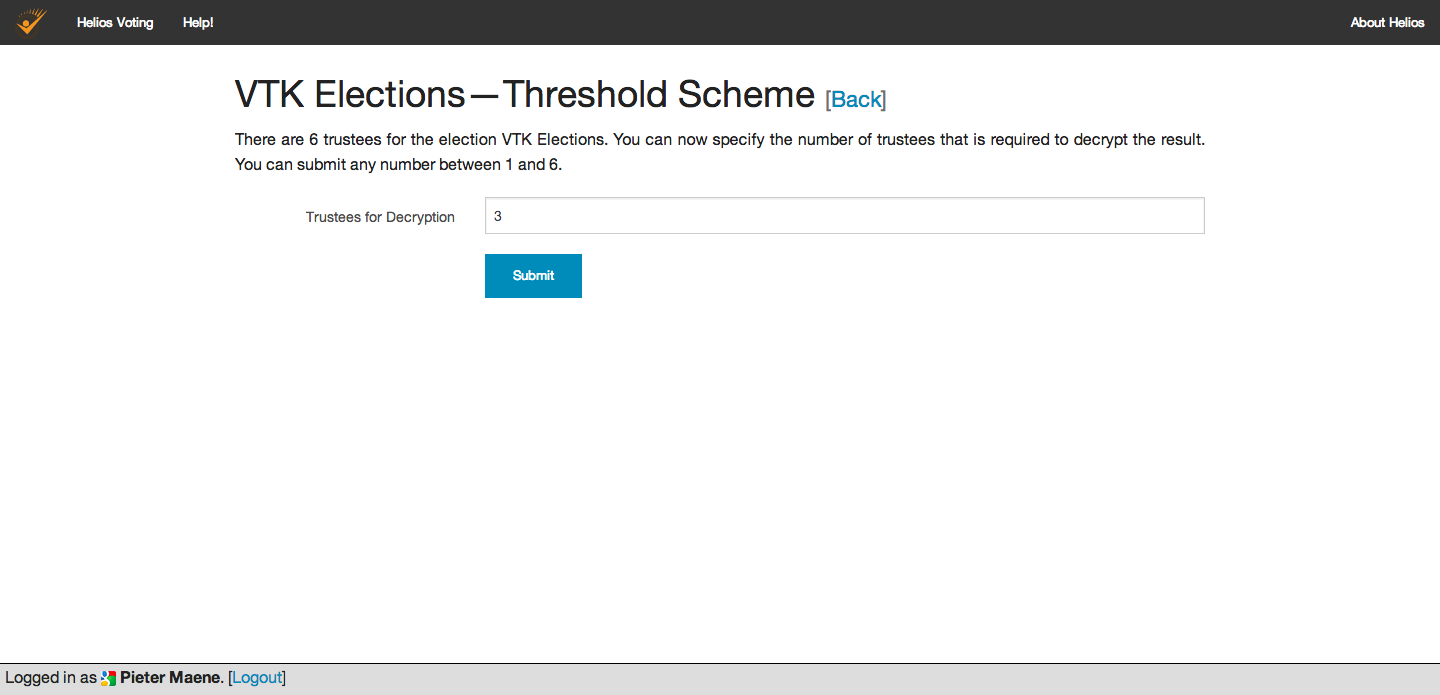
\includegraphics[width=0.9\linewidth]{proc/trustees_freeze.png}}
  \caption{Threshold Scheme}
  \label{fig:proc:trustees_freeze}
\end{figure}

%TODO Referentie naar Threshold Encryptie in Helios

\begin{enumerate}
  \item De trustees moeten eerst de twee sleutelparen genereren die gebruikt zullen worden om hun onderlinge communicatie te beveiligen. Pas wanneer alle trustees deze stap uitgevoerd hebben, kan verdergegaan worden.
  \item Elke trustee maakt vervolgens zijn shares aan en encrypteert deze voor de andere trustees. Hier moet opnieuw gewacht worden totdat alle trustees deze stap voltooid hebben.
  \item De trustees kunnen nu de shares die ze van de andere gekregen hebben decrypteren en optellen. Zo bekomen ze het sleutelpaar dat later gebruikt zal kunnen worden om de encryptiesleutel van de verkiezing de reconstrueren.
\end{enumerate}

Pas wanneer alle trustees de volledige sleutelceremonie doorlopen hebben, kan de verkiezing door de beheerder bevroren worden. Omdat de verschillende trustees dus vaak op elkaar moeten wachten, krijgen ze een e-mail elke keer de volgende stap uit de ceremonie aangevat kan worden. Tijdens het wachten op de trustees, kan de beheerder verdergaan met de procedure.

\subsection{Vragen}

Terwijl de trustees bezig zijn met het uitvoeren van de sleutelceremonie, kan het stembiljet wel aangemaakt worden. Alle informatie die hiervoor nodig is, werd reeds voorbereid (\ref{sec:proc:voorbereiding:vragen}).

\begin{figure}
  \center{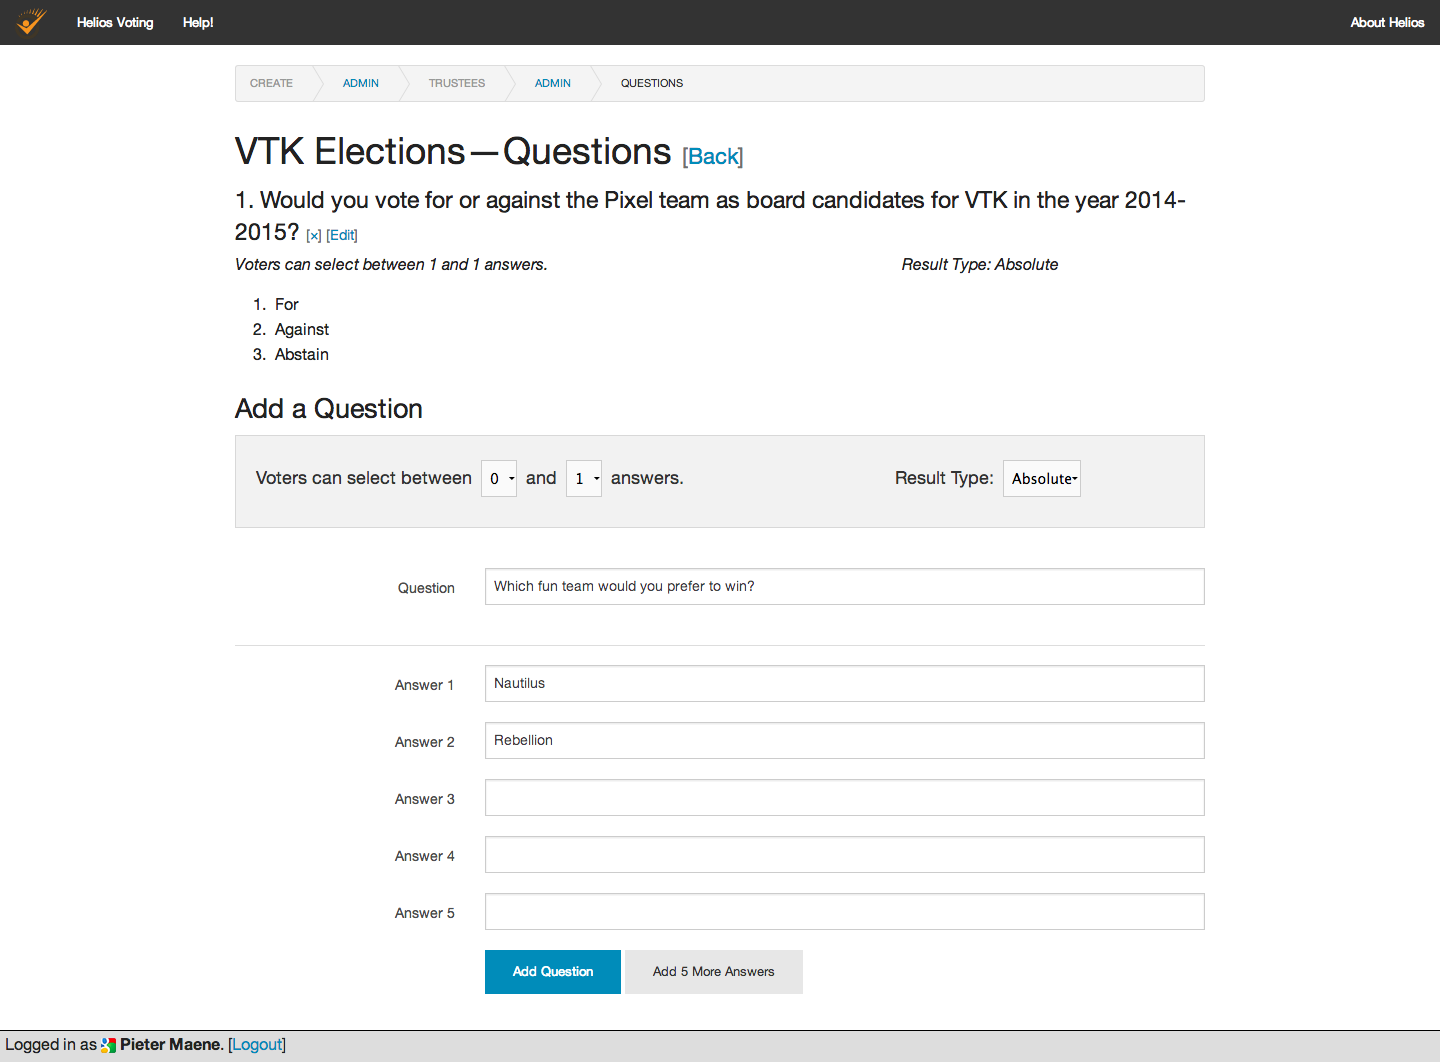
\includegraphics[width=0.9\linewidth]{proc/questions.png}}
  \caption{Questions}
  \label{fig:proc:questions}
\end{figure}

\subsection{Kiezers}

Ook deze stap werd reeds volledig voorbereid (\ref{sec:proc:voorbereiding:vragen}). Hier kunnen de voorbereidde de CSV-bestanden ge\"upload worden, waarna het systeem ze verwerkt en alle kiezers toevoegt aan de verkiezing.

\begin{figure}
  \center{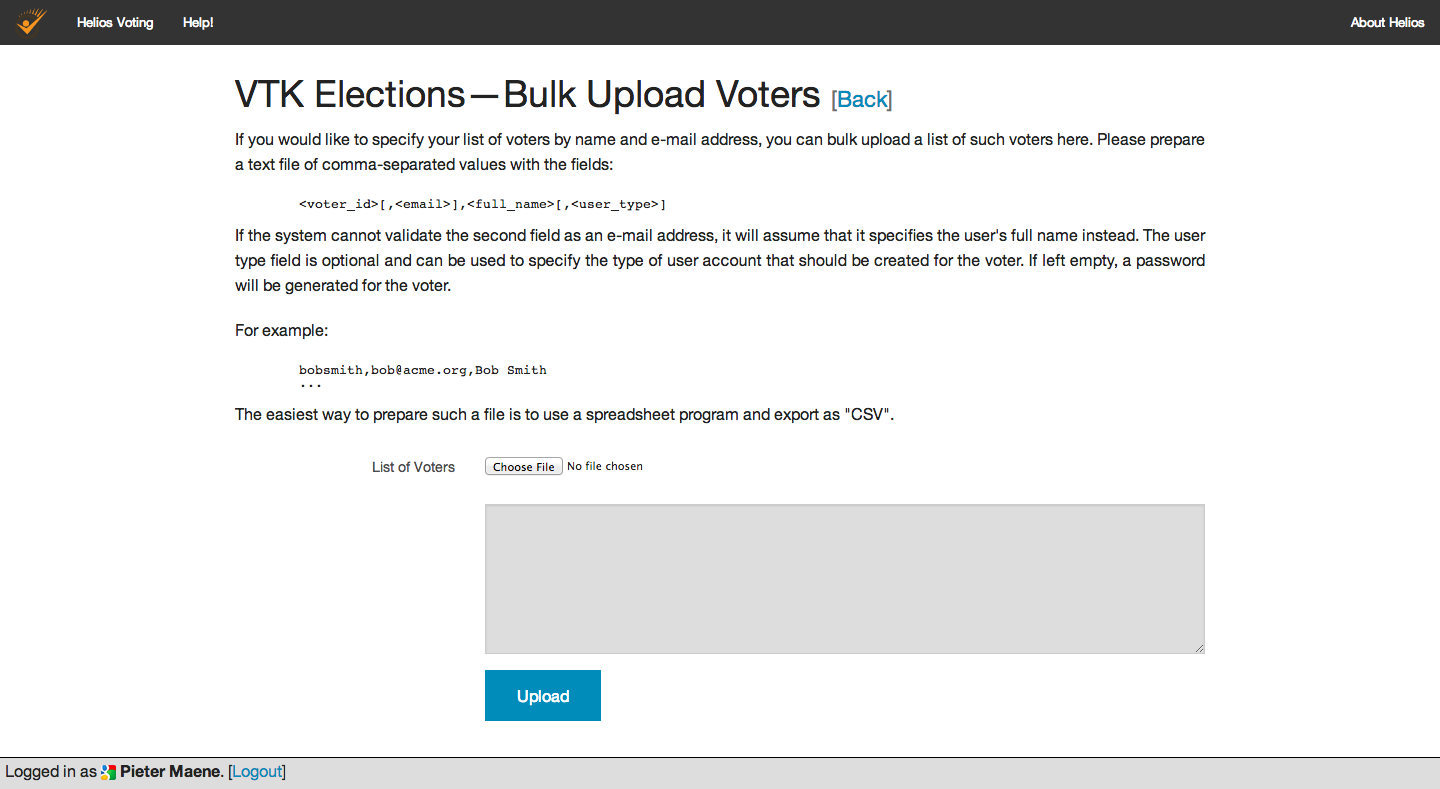
\includegraphics[width=0.9\linewidth]{proc/voters_upload.png}}
  \caption{Bulk Upload Voters}
  \label{fig:proc:voters_upload}
\end{figure}

\subsection{Bevriezen van het stembilhet}

Wanneer alle voorgaande informatie ingegeven is en de sleutelceremonie afgerond is, kan het stembiljet bevroren worden. Wanneer er geen tijdsstip gegeven is waarop de verkiezing moet starten, kunnen de kiezers onmiddellijk beginnen stemmen. Wanneer geen einddatum opgegeven is, blijft ze open totdat de beheerder ze sluit.

\subsection{Telling}

%TODO Referentie naar Homomorfisme in Helios

De stemming kan steeds manueel afgesloten worden door het telproces te starten. De stemmen worden dan homomorf samengeteld in een geëncrypteerd resultaat. Vooraleer dit gedecrypteerd kan worden, moeten we opnieuw wachten op de trustees.

\npar Wanneer geen threshold encryptie gebruikt wordt, moeten alle trustees nu hun decryptiefactor berekenen en uploaden. Wordt dit wel gebruikt, dan moeten slechts $k$ van de $n$ trustees dit doen. Zodra alle nodige decryptiefactoren beschikaar zijn, kan de beheerder het resultaat vrijgeven. Indien geen publicatiedatum opgegeven werd, is het resultaat dan voor iedereen beschikbaar. Anders kan de beheerder het resultaat wel reeds bekijken, maar wordt het pas gepubliceerd op die datum.

\begin{figure}
  \center{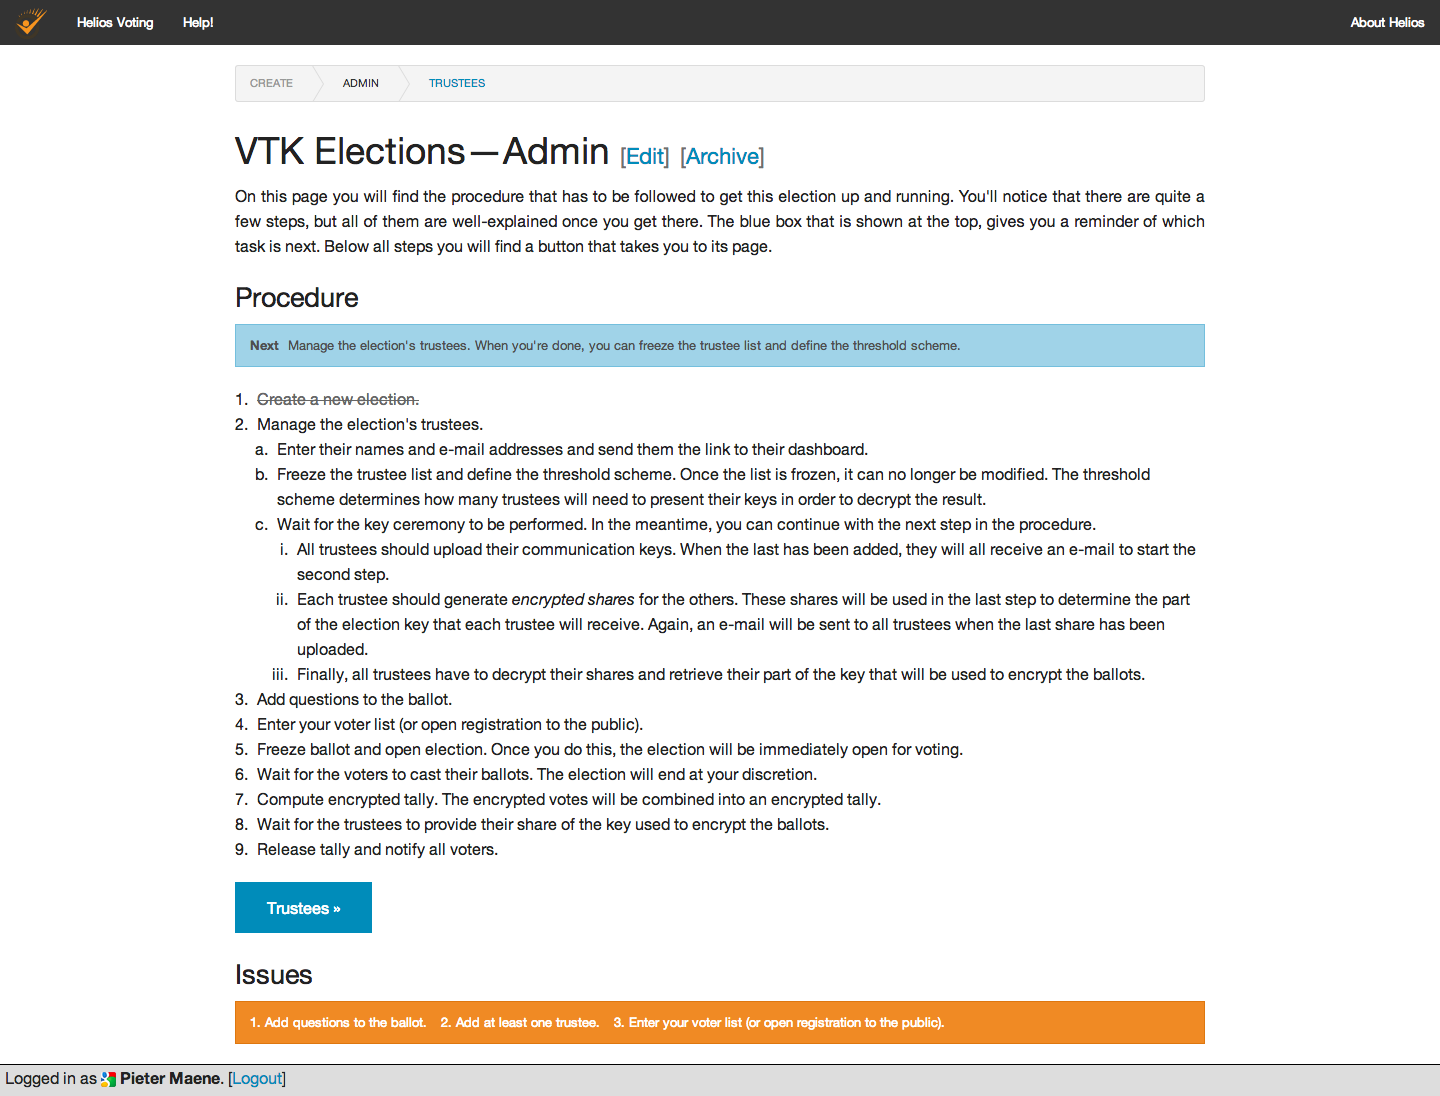
\includegraphics[width=0.9\linewidth]{proc/elections_admin.png}}
  \caption{Admin}
  \label{fig:proc:elections_admin}
\end{figure}
